\newcommand\Ksym{K_\mathsf{sym}}
\newcommand\Kfhe{K_\mathsf{FHE}}
\newcommand\Kspacesym{\mathcal{K}_\mathsf{sym}}
\newcommand\Kspacefhe{\mathcal{K}_\mathsf{FHE}}

  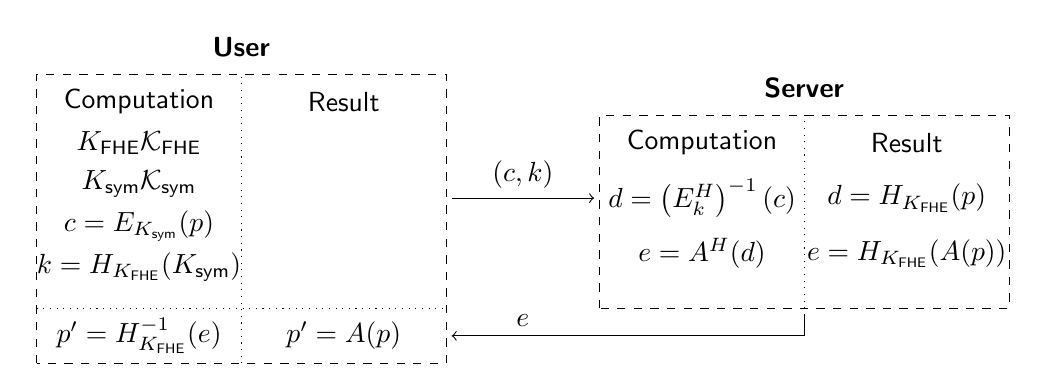
\begin{tikzpicture}[xscale=1.3,yscale=0.35]
    % User
    \draw (1, 9.5) node{\textbf{\textsf{User}}};
    \draw[dashed] (-1, -2) rectangle (3, 8.5) ;
    \draw (0, 7.5) node{\textsf{Computation}};
    \draw (2, 7.5) node{\textsf{Result}};
    \draw[dotted] (1, -2) -- (1, 8.5);
    \draw (0, 6) node{$\Kfhe \drawfrom \Kspacefhe$} ;
    \draw (0, 4.5) node{$\Ksym \drawfrom \Kspacesym$} ;
    \draw (0, 3) node{$c = E_{\Ksym}(p)$} ;
    \draw (0, 1.5) node{$k = H_{\Kfhe}(\Ksym)$} ;
    \draw[dotted] (-1, 0) -- (3, 0);
    \draw (0, -1) node{$p' = H_{\Kfhe}^{-1}(e)$};
    \draw (2, -1) node{$p' = A(p)$};
    % Server
    \draw (6.5, 8) node{\textbf{\textsf{Server}}} ;
    \draw[dashed]  (4.5, 0) rectangle (8.5, 7);
    \draw (5.5, 6) node{\textsf{Computation}};
    \draw (7.5, 6) node{\textsf{Result}};
    \draw[dotted] (6.5, 0) -- (6.5, 7);
    \draw (5.5, 4) node{ $d = \left(E^H_k\right)^{-1}(c)$ };
    \draw (7.5, 4) node{ $d = H_{\Kfhe}(p)$ };
    \draw (5.5, 2) node{ $e = A^H(d)$ };
    \draw (7.5, 2) node{ $e = H_{\Kfhe}(A(p))$ };
    %\draw (6, 1.5) node{ $f = E^H_k(d)$ };
    % arrows
    \draw[->,shorten >=2pt,shorten <=2pt] (3, 4) -- (4.5, 4) node[above,pos=0.5]{$(c, k)$} ;
    \draw[->,shorten >=2pt,shorten <=2pt] (6.5, 0) -- (6.5, -1) -- (3, -1) node[above,pos=0.786]{$e$};
  \end{tikzpicture}
  \caption{\label{fig:transciphering-principle} The principle of transciphering, where $E$ is a symmetric cipher (with secret key $\Ksym$ sampled from the space $\Kspacesym$), $H$ is a fully homomorphic cipher (with private key $\Kfhe$ sampled from the space $\Kspacefhe$), $E^H$ is a homomorphic evaluation of $E$, $A$ corresponds to some arbitrary operations, and $A^H$ to their homomorphic evaluation. %\nicolas{Il y a un souci avec la troisième ligne du serveur non ? Ca n'a pas de sens rechiffrer avec Transistor les chiffrés TFHE. Pour le sens "retour" les techniques sont différentes (cf eprint.iacr.org/2024/1921 par exemple). Je pense qu'il vaut mieux ne pas le mettre}\lp{c'est implémenté}
    % \jb{Les deux $f$ sont à remplacer par des $e$, non ?}\lp{oui je pense}
    % \lp{diagramme et légende mis à jour pour prendre en compte tous les commentaires, à vérifier donc}
    %\gl{J'ai séparé les calcul et les implications, et j'ai remplacé $p' = E^{-1}_{\Ksym}(e)$ par $p' = H_{\Kfhe}^{-1}(e)$}
    %\nicolas{J'ai rajouté la génération de clé FHE; et j'ai remplacé par des notations génériques pour els espaces de clé (on n'a pas encore introduit que Transistor marche dans $\mainField$)}
    %\gl{Si on veux ajouter la clef FHE dans le schema, il faut transferer la clef publique, non?}
  }

